\chapter{Diseño e implementación}
\label{chap:diseno}



\section{Herramientas empleadas}
\label{sec:HerramientasEmpleadas}


\subsection{Unity 6}
\label{subsec:Unity6}

//TODO: plataforma de desarrollo de videojuegos...


\clearpage

\subsection{GitHub y Git}
\label{subsec:GitHubGit}

GitHub es una plataforma web de alojamiento principalmente de código fuente de proyectos de carácter  colaborativo. Basa su funcionamiento en Git, uno de los sistemas de control de versiones por excelencia, permitiendo realizar un seguimiento de los cambios en los archivos. Es de especial utilidad en entornos de trabajo colaborativo en los cuales varias personas pueden estar trabajando simultáneamente en el mismo proyecto e ir realizando cambios en los ficheros y subirlos de manera independiente (orden \texttt{commit}) para, posteriormente, juntar esos cambios (orden \texttt{merge}) \cite{GitHub}.

Además, es excelente para llevar una trazabilidad exhaustiva de los cambios generados en cada fichero, de tal forma que se pueden generar versiones del proyecto en las que se vayan creando nuevas funcionalidades o solucionando problemas detectados. De hecho, es recomendable crear ramas (orden \texttt{branch}) para cada paquete de trabajo lo suficientemente diferente del resto, como solución de problemas o cada nueva funcionalidad, de tal forma que al terminarlo se una a la rama principal.

Para este caso concreto, se ha trabajado sobre dos repositorios de GitHub, donde se han ido subiendo los cambios tanto de la aplicación como de este propio documento:

\begin{itemize}

	\bigskip
	\item Aplicación <<ATC Analysis and Training Tool>> desarrollada en el marco de este trabajo:
	
	\begin{itemize}
		\item Repositorio: \url{https://github.com/macgyver912/atc-simulator}
		\item Ramas: \texttt{master} y \texttt{jaime} (donde está todo el desarrollo).
		\item Colaboradores: usuario \href{https://github.com/macgyver912}{\textit{macgyver912}} (Jaime Valle Alonso).
	\end{itemize}
	
	\bigskip
	\begin{figure}[!hbtp]
		\centering
		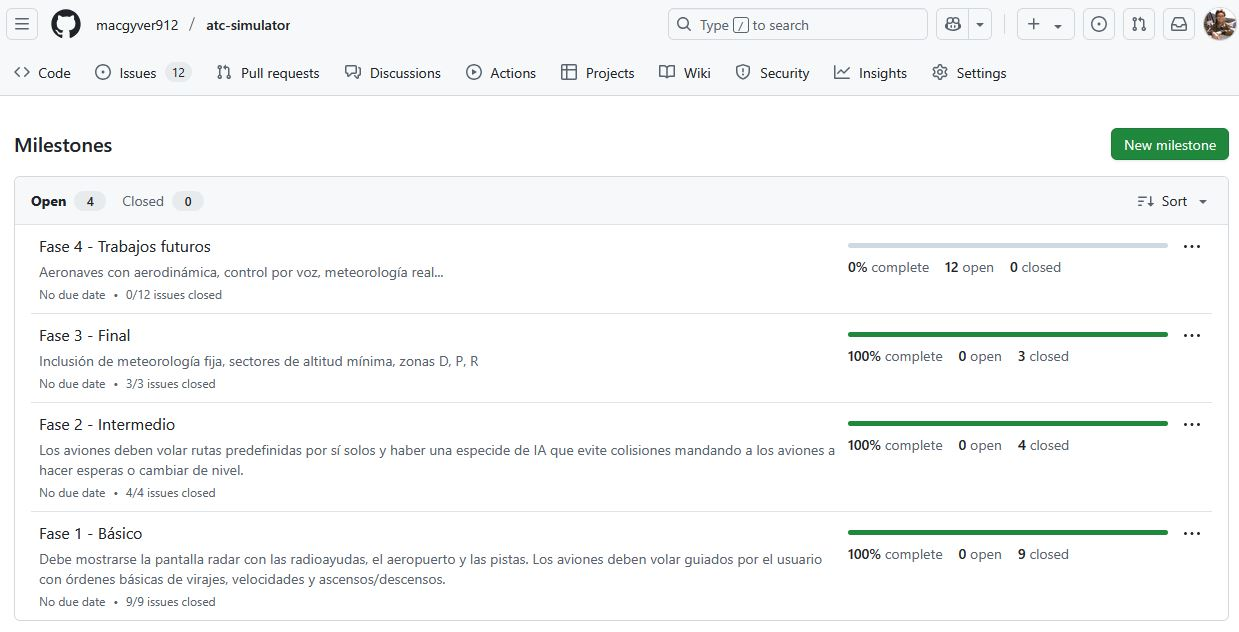
\includegraphics[width=1.0\linewidth]{images/content/GitHub_Aplicacion_Milestones.jpg}
		\caption{Repositorio de <<ATC Analysis and Training Tool>>.}
		\label{fig:GitHub_Aplicacion_Milestones}
	\end{figure}	
	
	\pagebreak
	
	
	\bigskip
	\item Elaboración de la memoria, este propio documento:
	
	\begin{itemize}
		\item Repositorio: \url{https://github.com/macgyver912/urjc-tfg}
		\item Ramas: \texttt{master} y \texttt{jaime} (donde está todo el desarrollo).
		\item Colaboradores: usuario \href{https://github.com/macgyver912}{\textit{macgyver912}} (Jaime Valle Alonso).
	\end{itemize}
	
	En la Figura \ref{fig:GitTFG} se muestran los comandos empleados para subir los cambios al repositorio remoto, que son los siguientes:
	
	\begin{itemize}
		\item \texttt{git status}: muestra los ficheros que se han modificado9 desde el último \texttt{commit}.
		
		\item \texttt{git add -u}: prepara todos los ficheros modificados para subir en próximo \texttt{commit}.
		
		\item \texttt{git commit -m}: establece la cabecera de modificaciones al estado actual de tal forma que los ficheros que se añadieron ahora son la versión actual para el proyecto. El modificador \texttt{-m} se emplea para añadir un comentario descriptivo de los cambios.
		
		\item \texttt{git push origin jaime}: sube los cambios al repositorio que está en la web de GitHub, concretamente a la rama \texttt{jaime} (lo anterior sólo estaba en local).
	\end{itemize}	 	
	
	\bigskip
	\begin{figure}[!hbtp]
		\centering
		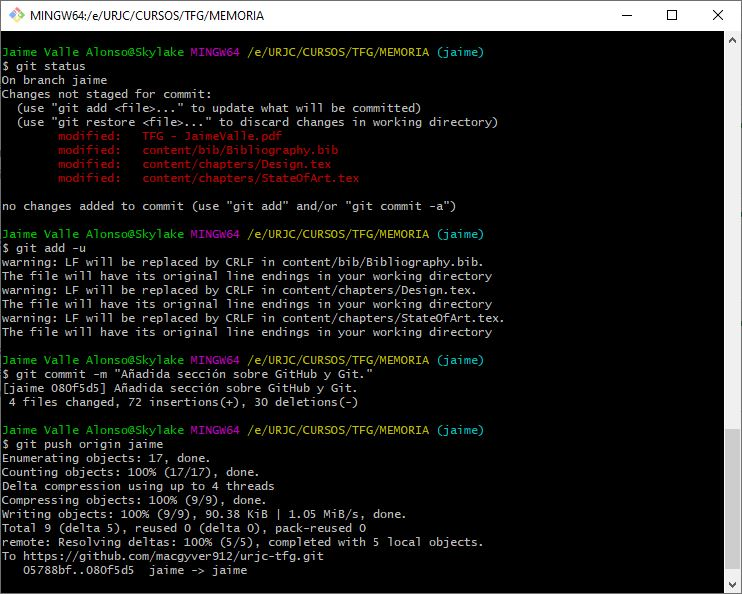
\includegraphics[width=0.9\linewidth]{images/content/GitTFG.jpg}
		\caption{Comandos para subir cambios al repositorio de la memoria en GitHub.}
		\label{fig:GitTFG}
	\end{figure}	
		
	
\end{itemize}


\clearpage

\subsection{GIMP}
\label{subsec:GIMP}

//TODO: empleado para iconos...

\clearpage

\subsection{\LaTeX y Texmaker}
\label{subsec:LaTeX_Texmaker}

\LaTeX es un sistema multiplataforma de composición de textos de alta calidad, diseñado y ampliamente empleado para la publicación de documentos científicos y técnicos. Esto se debe a la facilidad de escribir ecuaciones y símbolos matemáticos a partir de comandos de texto, sin necesidad de recurrir a y submenús como ocurre en otras aplicaciones. Además es gratuito y de código abierto \cite{latex}.

Si bien, es una muy potente, requiere de cierto tiempo para que el usuario aprenda desenvolverse con él, principalmente debido a que no se trata de una herramienta WYSIWYG (\textit{What You See Is What You Get}). Esto es, el formato aplicado al documento de texto que se está generando no se ve mientras se edita, sino que necesita compilarse. 

Por ello, \LaTeX debe verse como una herramienta que está entre programación y editor de texto. Si bien emplea comandos sencillos, la infinidad de posibilidades que ofrece, puede llegar a abrumar a los que comienzan con ello. Pero nada más lejos de la realidad; es una herramienta muy útil y que simplifica muchas tareas.

Al tener esa componente de comandos con guiños hacia la programación, pueden crearse variables y emplearlas para realizar cálculos, aplicar reglas condicionales a ciertos elementos, etc. Sin ir más lejos, la numeración de los requisitos de la sección \textit{\ref{chap:objetivos} \nameref{chap:objetivos}} ha sido realizada mediante una variable que aumenta su valor en una unidad cada vez que se añade una tabla mediante los comandos que se muestran a continuación:

{\footnotesize
\begin{Verbatim}[frame=single]
\newcounter{Req_F1_index}
\setcounter{Req_F1_index}{1}

\begin{tabular}{|c|p{0.75\textwidth}|}			
  \hline
  \multicolumn{2}{|l|}{\cellcolor{gray!10}
  {\textbf{ID: Req.F1.\arabic{Req_F1_index}}}} 
  \stepcounter{Req_F1_index} % <- Increments by one variable 'Req_F1_index'
  \\ \hline		
  \cellcolor{gray!10}{\textbf{Título}} 
  & Proyección 2D. \\
  \cellcolor{gray!10}{\textbf{Desc.}} 
  & Modelo matemático que permita trasladar las coordenadas de los objetos 
  a representar a posiciones 2D en la pantalla. 
  \\ \hline		
\end{tabular}
\end{Verbatim}
}

\pagebreak

\begin{figure}[!hbtp]
	\centering
	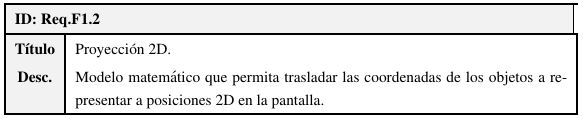
\includegraphics[width=0.8\linewidth]{images/content/latex_table.jpg}
	\caption{Tabla generada con la porción de código anterior.}
	\label{fig:latex_table}
\end{figure}	

Puesto que \LaTeX es una especie de lenguaje compilado, puede editarse como un fichero de texto plano desde cualquier editor y compilarse mediante el comando \texttt{latex}, de tal forma que, por defecto, generará un PDF con el contenido del documento.

No obstante, existen entornos de desarrollo apropiados para editar documentos \LaTeX, como {\TeX nicCenter} \cite{texniccenter} o Texmaker \cite{texmaker}. La apariencia general de ambos es muy similar, presentando tres grandes paneles verticales: el izquierdo como navegador de archivos del proyecto, el central como editor de texto plano y el derecho como visualizador del PDF generado. Si bien, poseen multitud de opciones para configurar, por lo que el usuario puede personalizar el entorno a su gusto.

\begin{figure}[!hbtp]
	\centering
	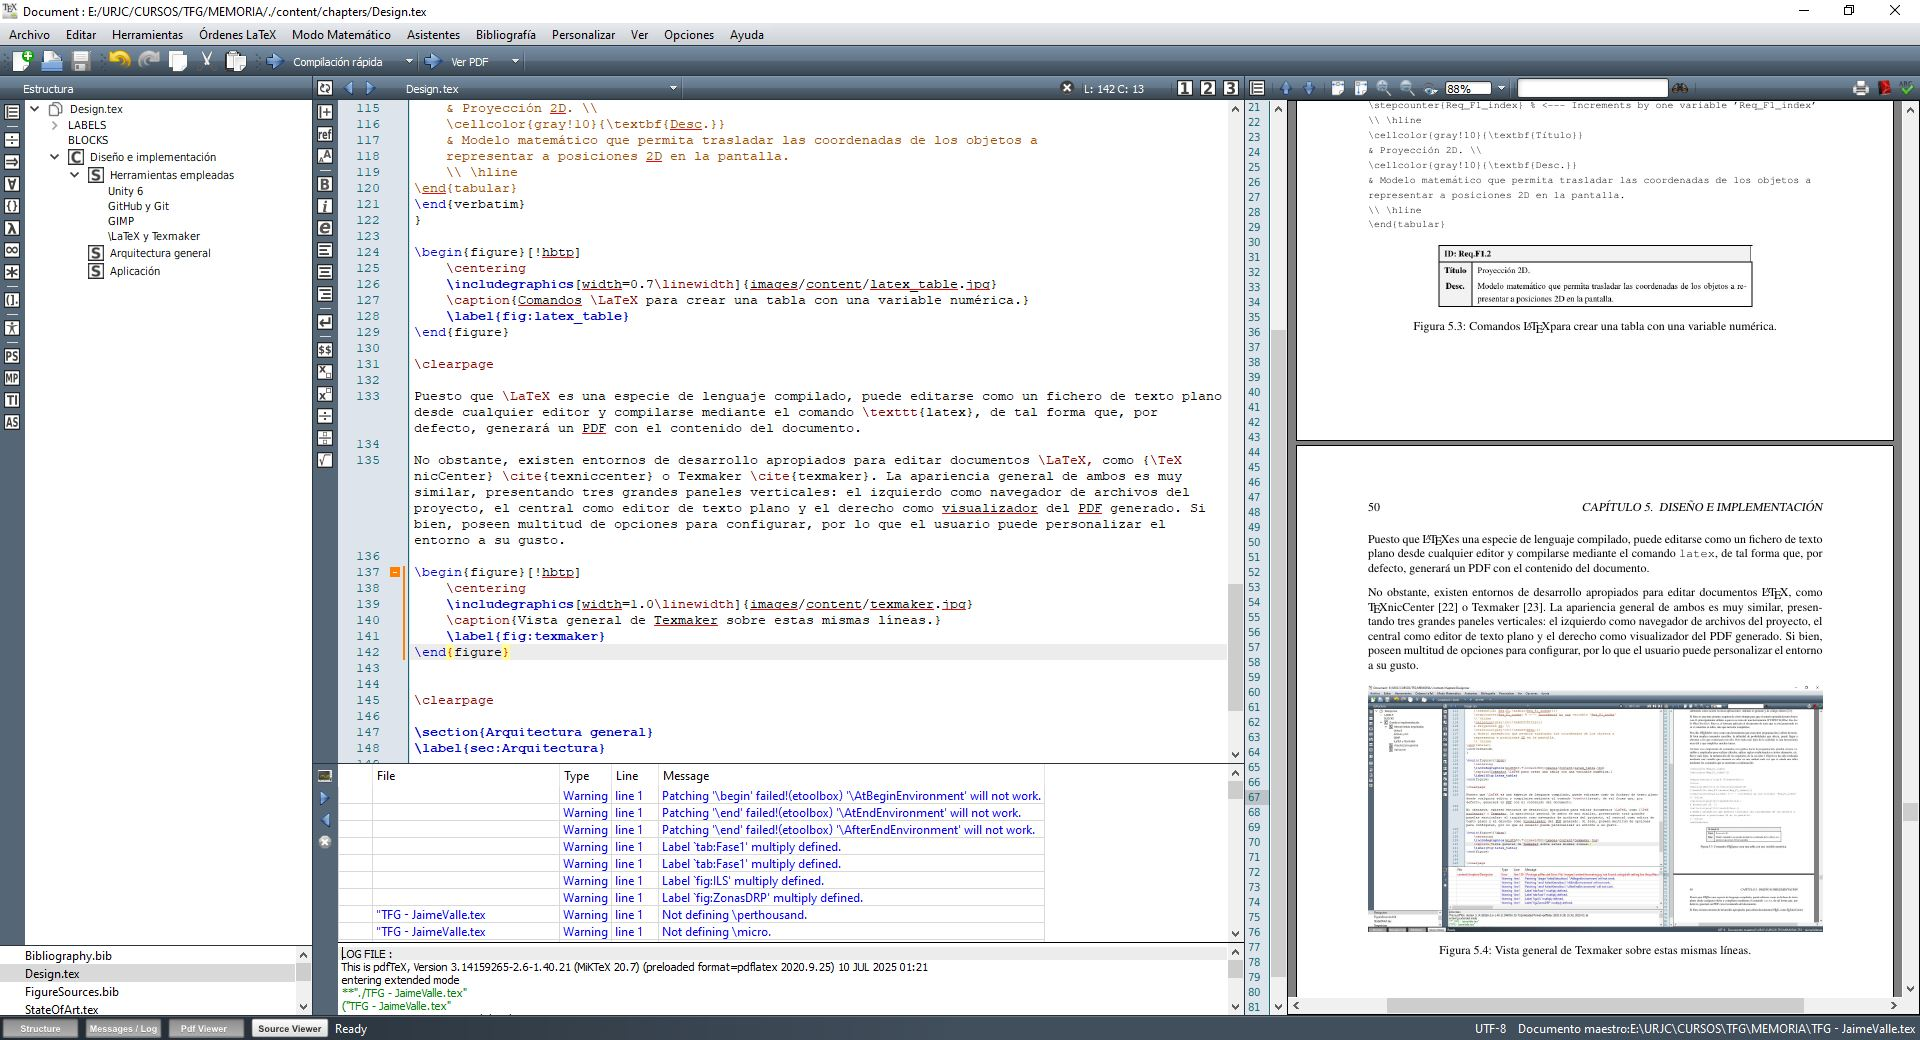
\includegraphics[width=1.0\linewidth]{images/content/texmaker.jpg}
	\caption{Vista general de Texmaker sobre estas mismas líneas.}
	\label{fig:texmaker}
\end{figure}


\clearpage

\section{Arquitectura general} 
\label{sec:Arquitectura}

//TODO: pantallazo o lista de puntos de directorios y ficheros de código fuente.

//TODO: breve descripción de cada una de las clases y sus miembros.


\section{Aplicación}
\label{sec:Aplicacion}

//TODO: pantallazos, descripción general...